\scanpage{53}
\deleted{$\unsure{G_1|G}$ \unsure{algébrique}}
\deleted{\figure{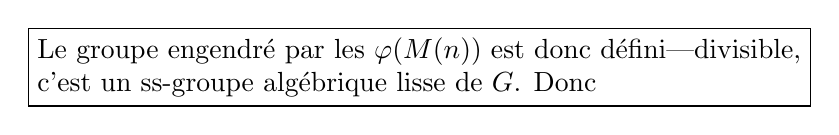
\begin{tikzpicture}\node[draw,align=left] {Le groupe engendré par les $\varphi(M(n))$ est donc \unsure{défini|divisible},\\c'est un ss-groupe algébrique lisse de $G$. Donc};\end{tikzpicture}}}

Supposons maintenant que $G$ soit un schéma en groupes Néronien sur un trait $S$ de corps de fonctions $K$, soit $M$ un groupe p-divisible, et $\varphi_K:M_K\mathbin{-}G_K$. Je dis que $\varphi_K$ se prolonge en $\varphi:M\longrightarrow G$ (évidemment unique).

Clair si $p\ne\operatorname{car.}$ résiduelle.

Supposons donc $p=\operatorname{car.}k$. Alors, ou bien $\operatorname{car.}K=p$, ou bien $\operatorname{car.}K=0$ (donc $K$ parfait); en tous cas, $G_K$ n'a pas de ss-groupe isom. à $G_a$, puisque $G_K$ admet un modèle de Néron. Donc on peut appliquer le lemme précédent, \deleted{Il existe} d'où un $H_K\subset G_K$ par lequel se factorise $\varphi$.

Comme $H_K$ est ext. d'une VA par un tore, $H_K$ admet un modèle de Néron $H$, et $H_K\xrightarrow{i_K}G_K$ est induit par $H\xrightarrow{i}K$. Le th. de Raynaud pour $H$ implique que $\psi_K:M_K\mathbin{-}H_K$ se prolonge en $\psi:M\longrightarrow H$. On gagne!

\mspage{52}
